\documentclass[aspectratio=169]{beamer}
\usepackage{simplebeamer}

\begin{document}

\begin{frame}

    \begin{center}
        \titletext{Coalescent inference of HIV transmission history}

        \vfill

        Raymond Heil
        
        T-6: Theoretical Biology and Biophysics

        \vspace{0.5cm}

        Mentors

        Emma Goldberg, Thomas Leitner, Ethan Romero-Severson

        \vfill

        \scriptsize{20 July 2022}

    \end{center}

    %\ftnA{LA-UR-XX-XXXXX} % add this back in when I get an LA-UR

\end{frame}

%--------------------------------------------------
\section{Why this project?}
%--------------------------------------------------

\begin{frame} \frametitle{\insertsection}

    \centering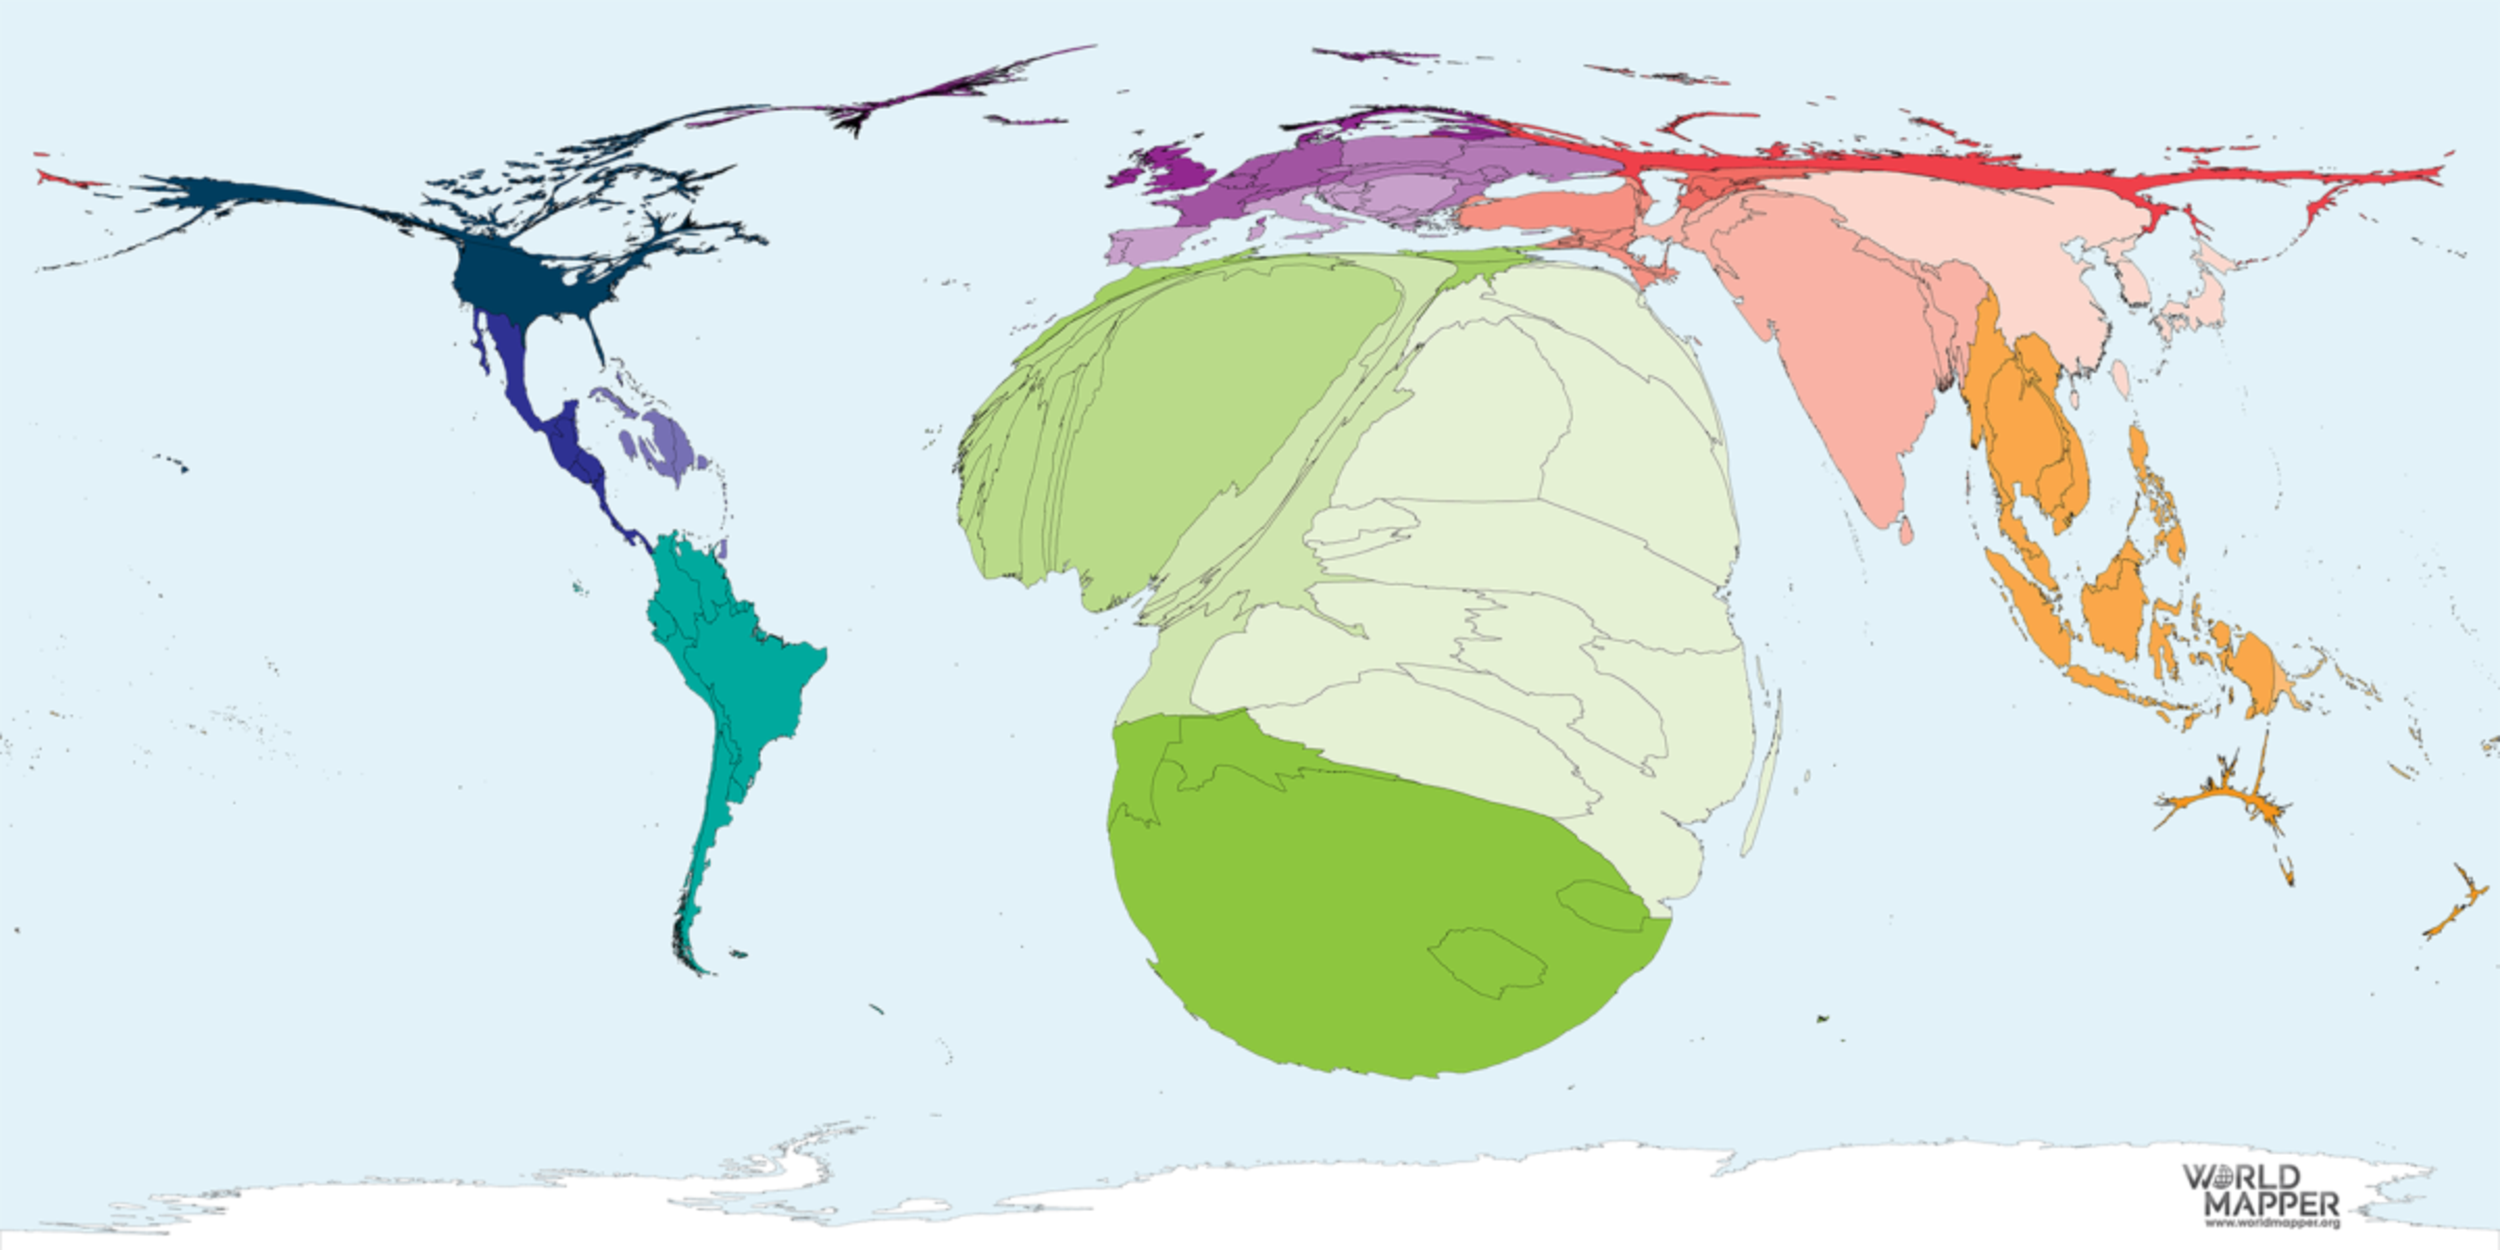
\includegraphics[width=0.65\textwidth]{images/hiv-cartogram}
    
    \begin{itemize}
        \item{HIV is globally widespread}
        \item{Despite effective therapy, it is still spreading}
        \item{How can we understand the way it spreads?}
    \end{itemize}

    \ftnB{Image from World Mapper, data from WHO Human Development Report (2013)}

\end{frame}

%-------------------------------------------------
\section{Setting up the problem}
%-------------------------------------------------

\begin{frame} \frametitle{\insertsection}
    \begin{center}
        \centering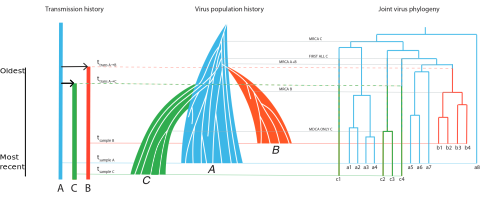
\includegraphics[width=\textwidth]{images/thomas-figure}
        \ftnB{Modified from Leitner et al., Curr. Opin. HIV AIDS (2019)}
    \end{center}
\end{frame}

%--------------------------------------------------
\section{Inferring information from a tree}
%--------------------------------------------------

\begin{frame} \frametitle{\insertsection}

    \begin{columns}

        \begin{column}{0.6\textwidth}
            
            \begin{center}
                \centering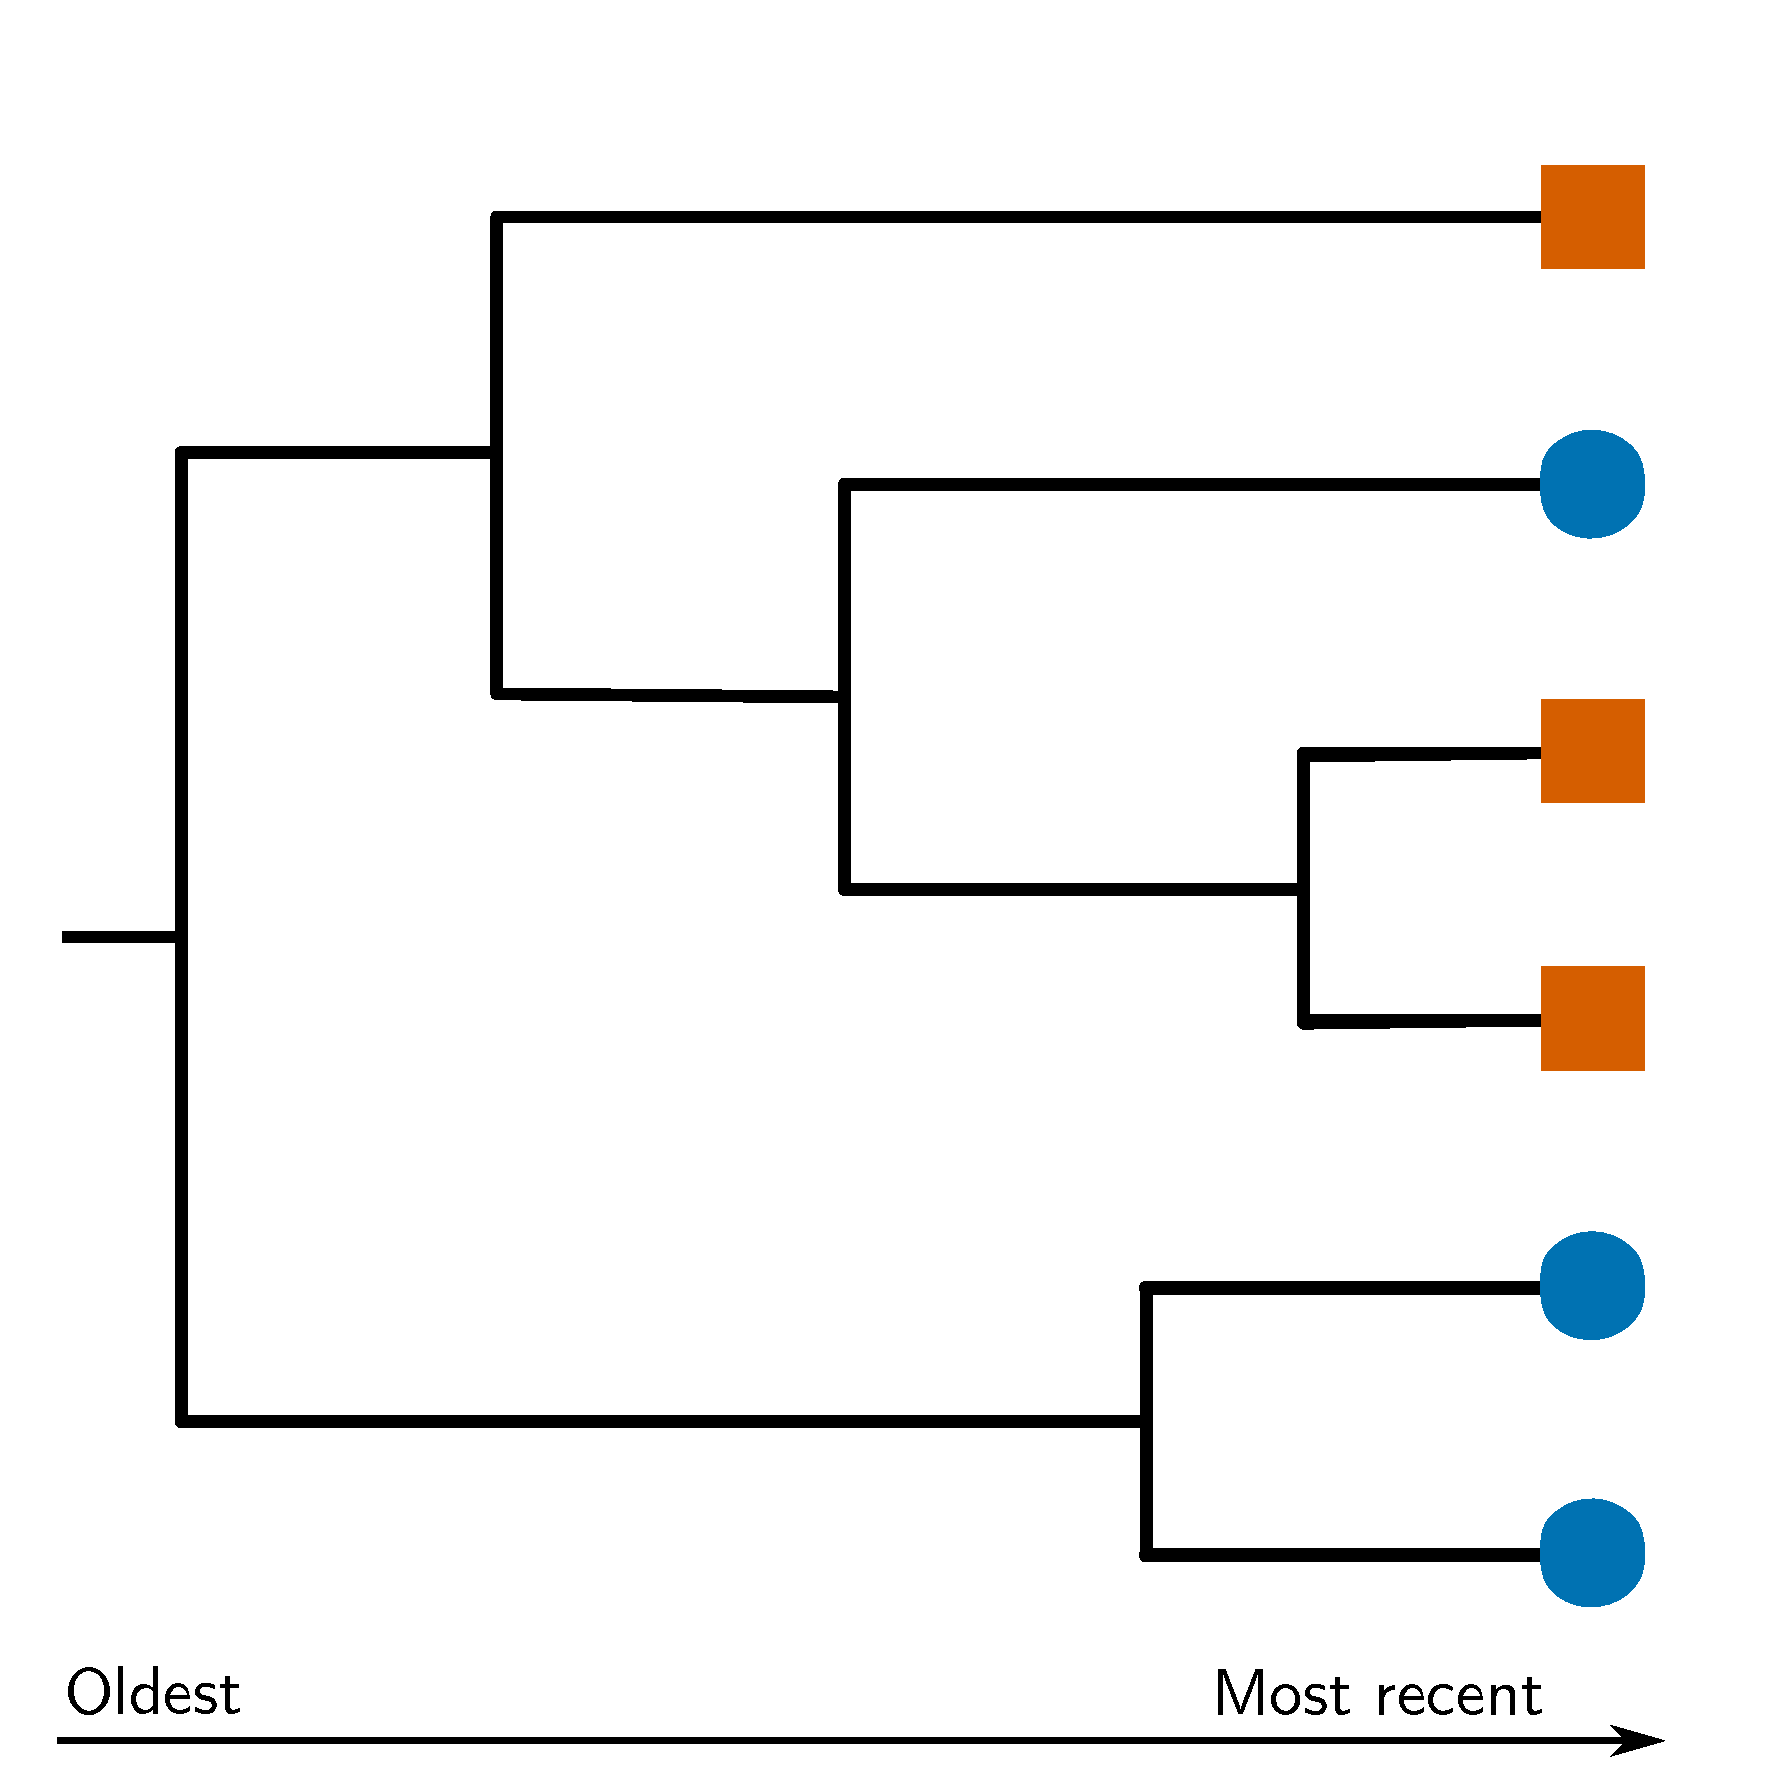
\includegraphics[width=0.8\textwidth]{images/tree-blank}
            \end{center}

        \end{column}

        \begin{column}{0.5\textwidth}

            \begin{itemize}
                \item{Tree tips represent \textbf{invividual viral sequences}}
                \item{Three samples from each invididual}
                \item{If one infected the other, when?}
            \end{itemize}

        \end{column}

    \end{columns}

\end{frame}

\begin{frame} \frametitle{\insertsection}

    \begin{center}

        \centering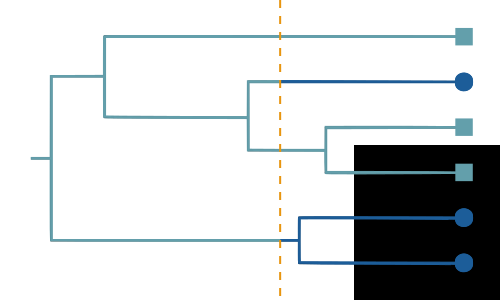
\includegraphics[width=0.8\textwidth]{images/tree-option1}
        
    \end{center}

\end{frame}


\begin{frame} \frametitle{\insertsection}

    \begin{center}

        \centering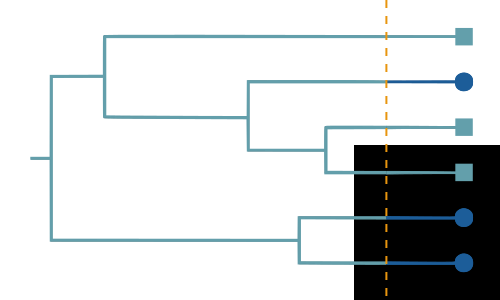
\includegraphics[width=0.8\textwidth]{images/tree-option2}

    \end{center}

\end{frame}


\begin{frame} \frametitle{\insertsection}

    \begin{center}

        \centering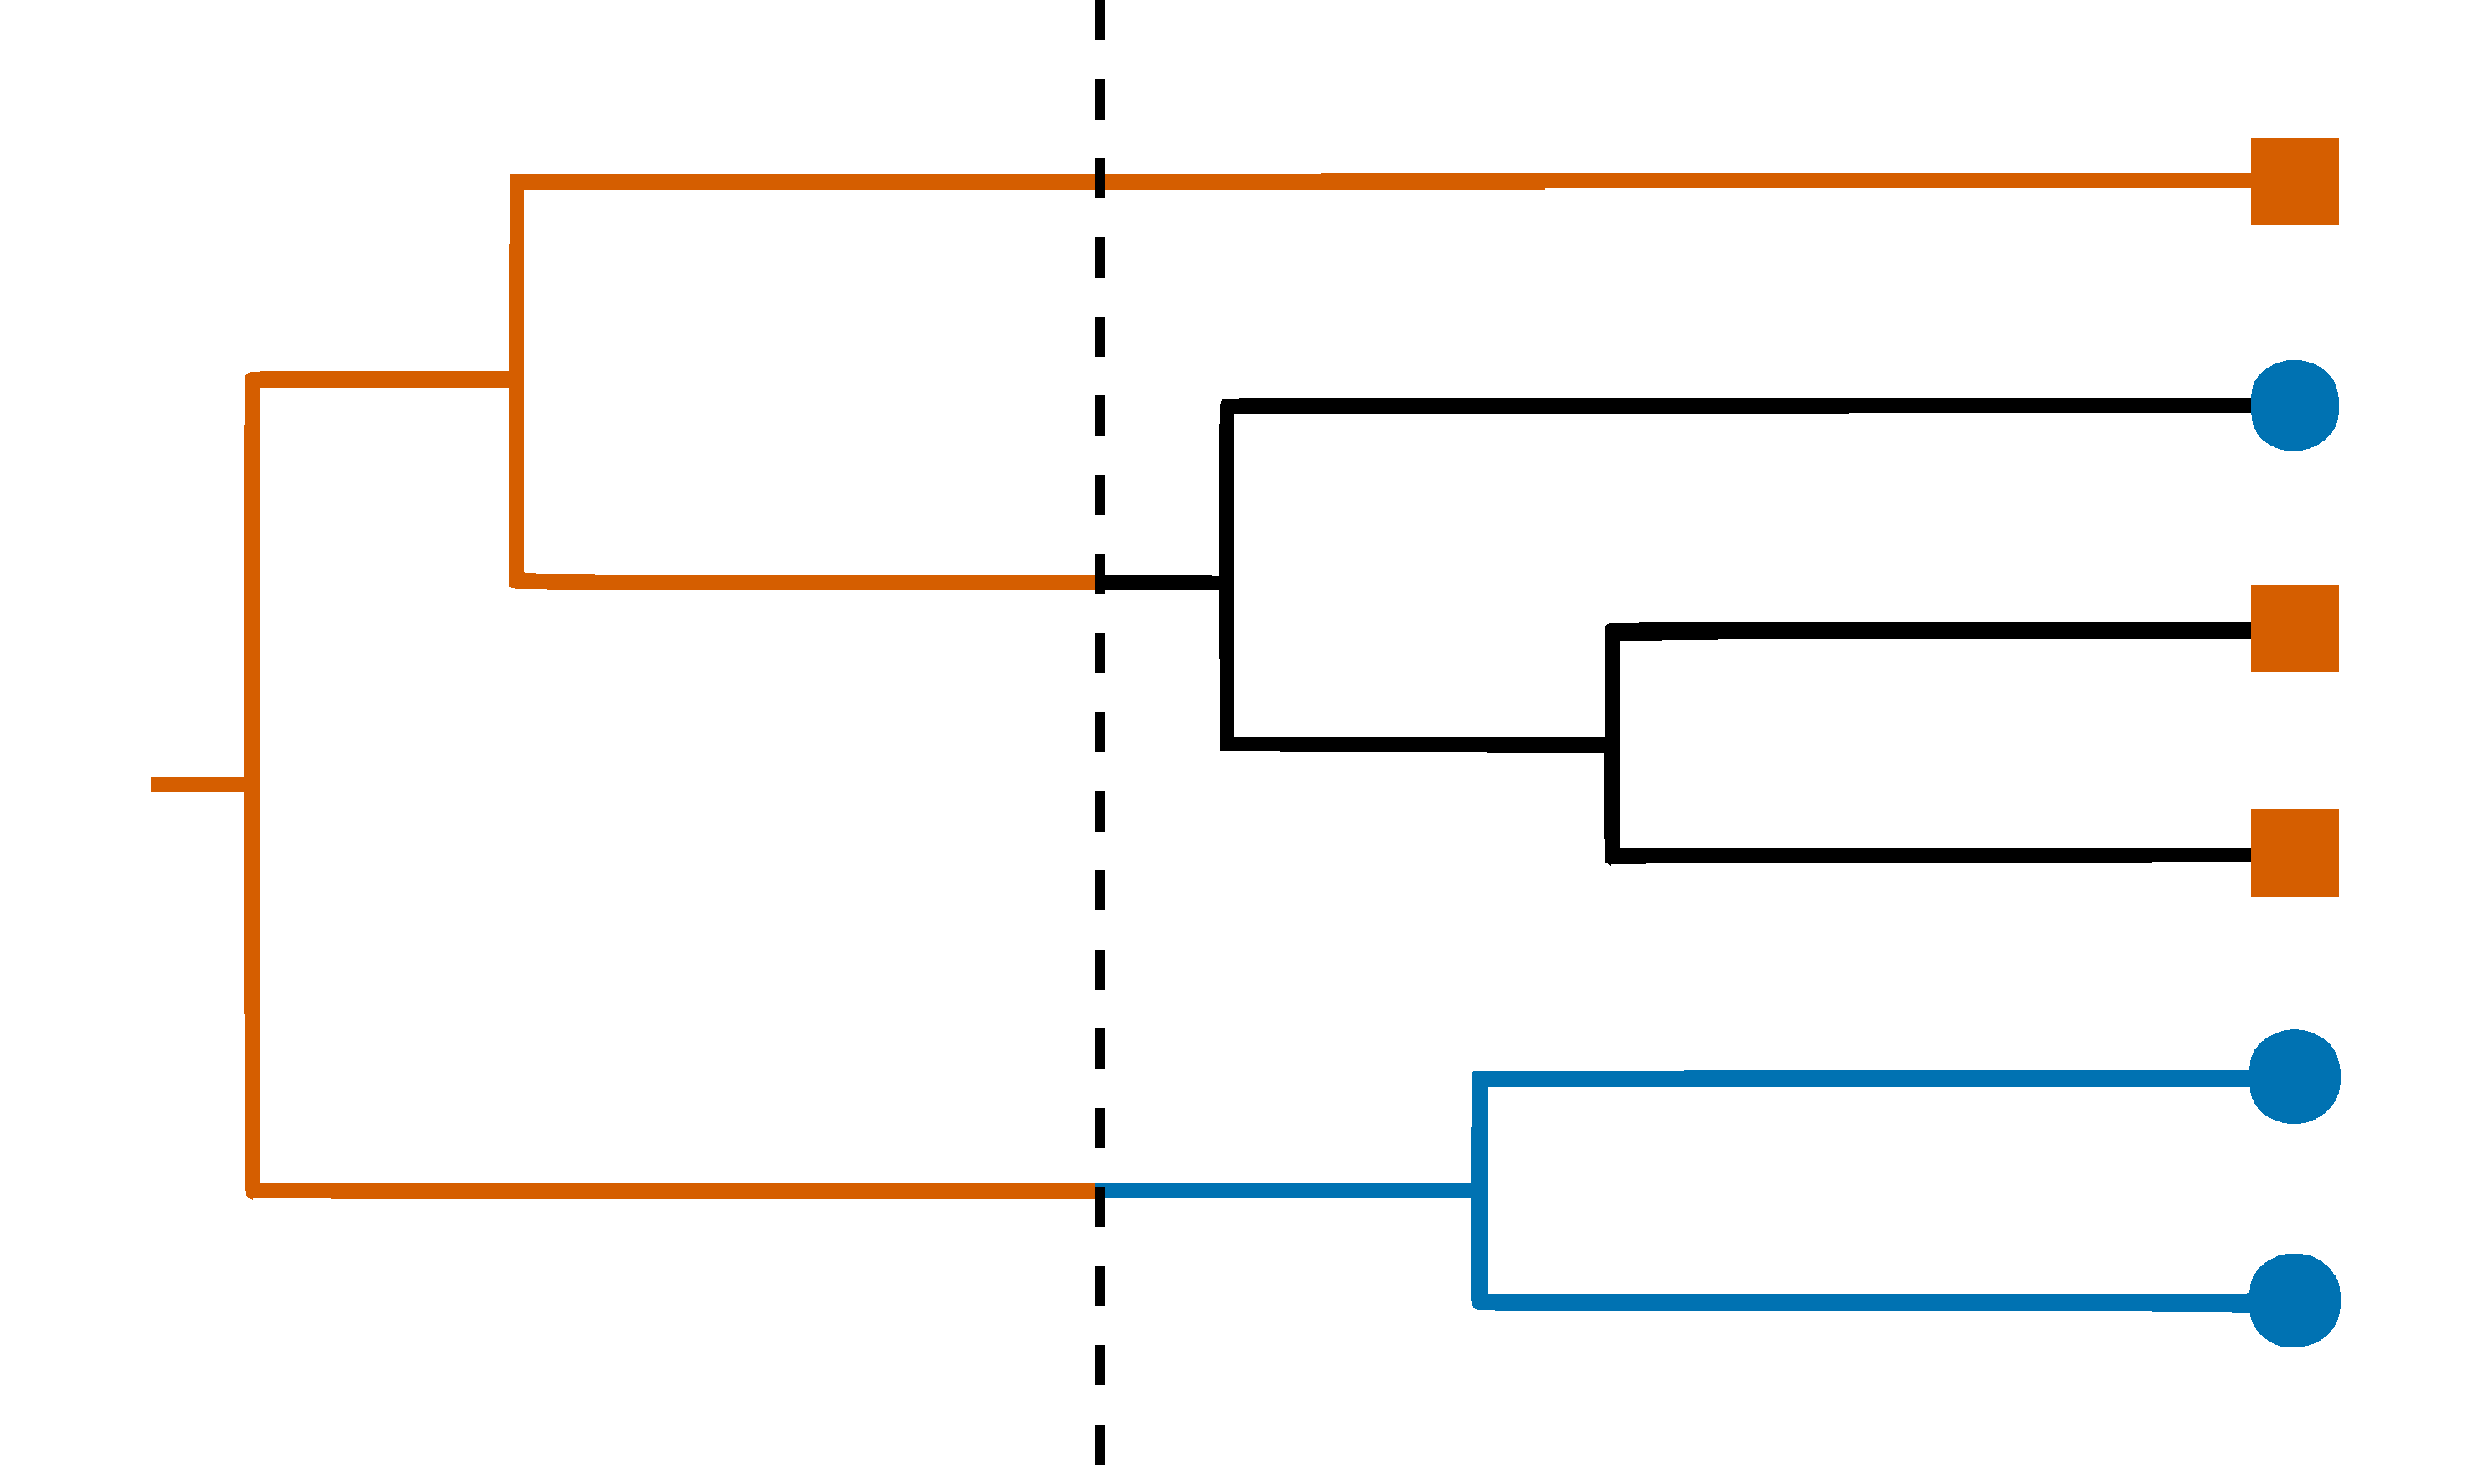
\includegraphics[width=0.8\textwidth]{images/tree-option3}

    \end{center}

\end{frame}


%--------------------------------------------------
\section{Coalescent modeling}
%--------------------------------------------------

\begin{frame} 
    \begin{center}
        \begin{huge}
    
            \textbf{Coalescent theory}

            Node times as a function of population size

        \end{huge}
    \end{center}
\end{frame}

%--------------------------------------------------
\section{Relationship between population and samples}
%--------------------------------------------------

\begin{frame} \frametitle{\insertsection}

        \centering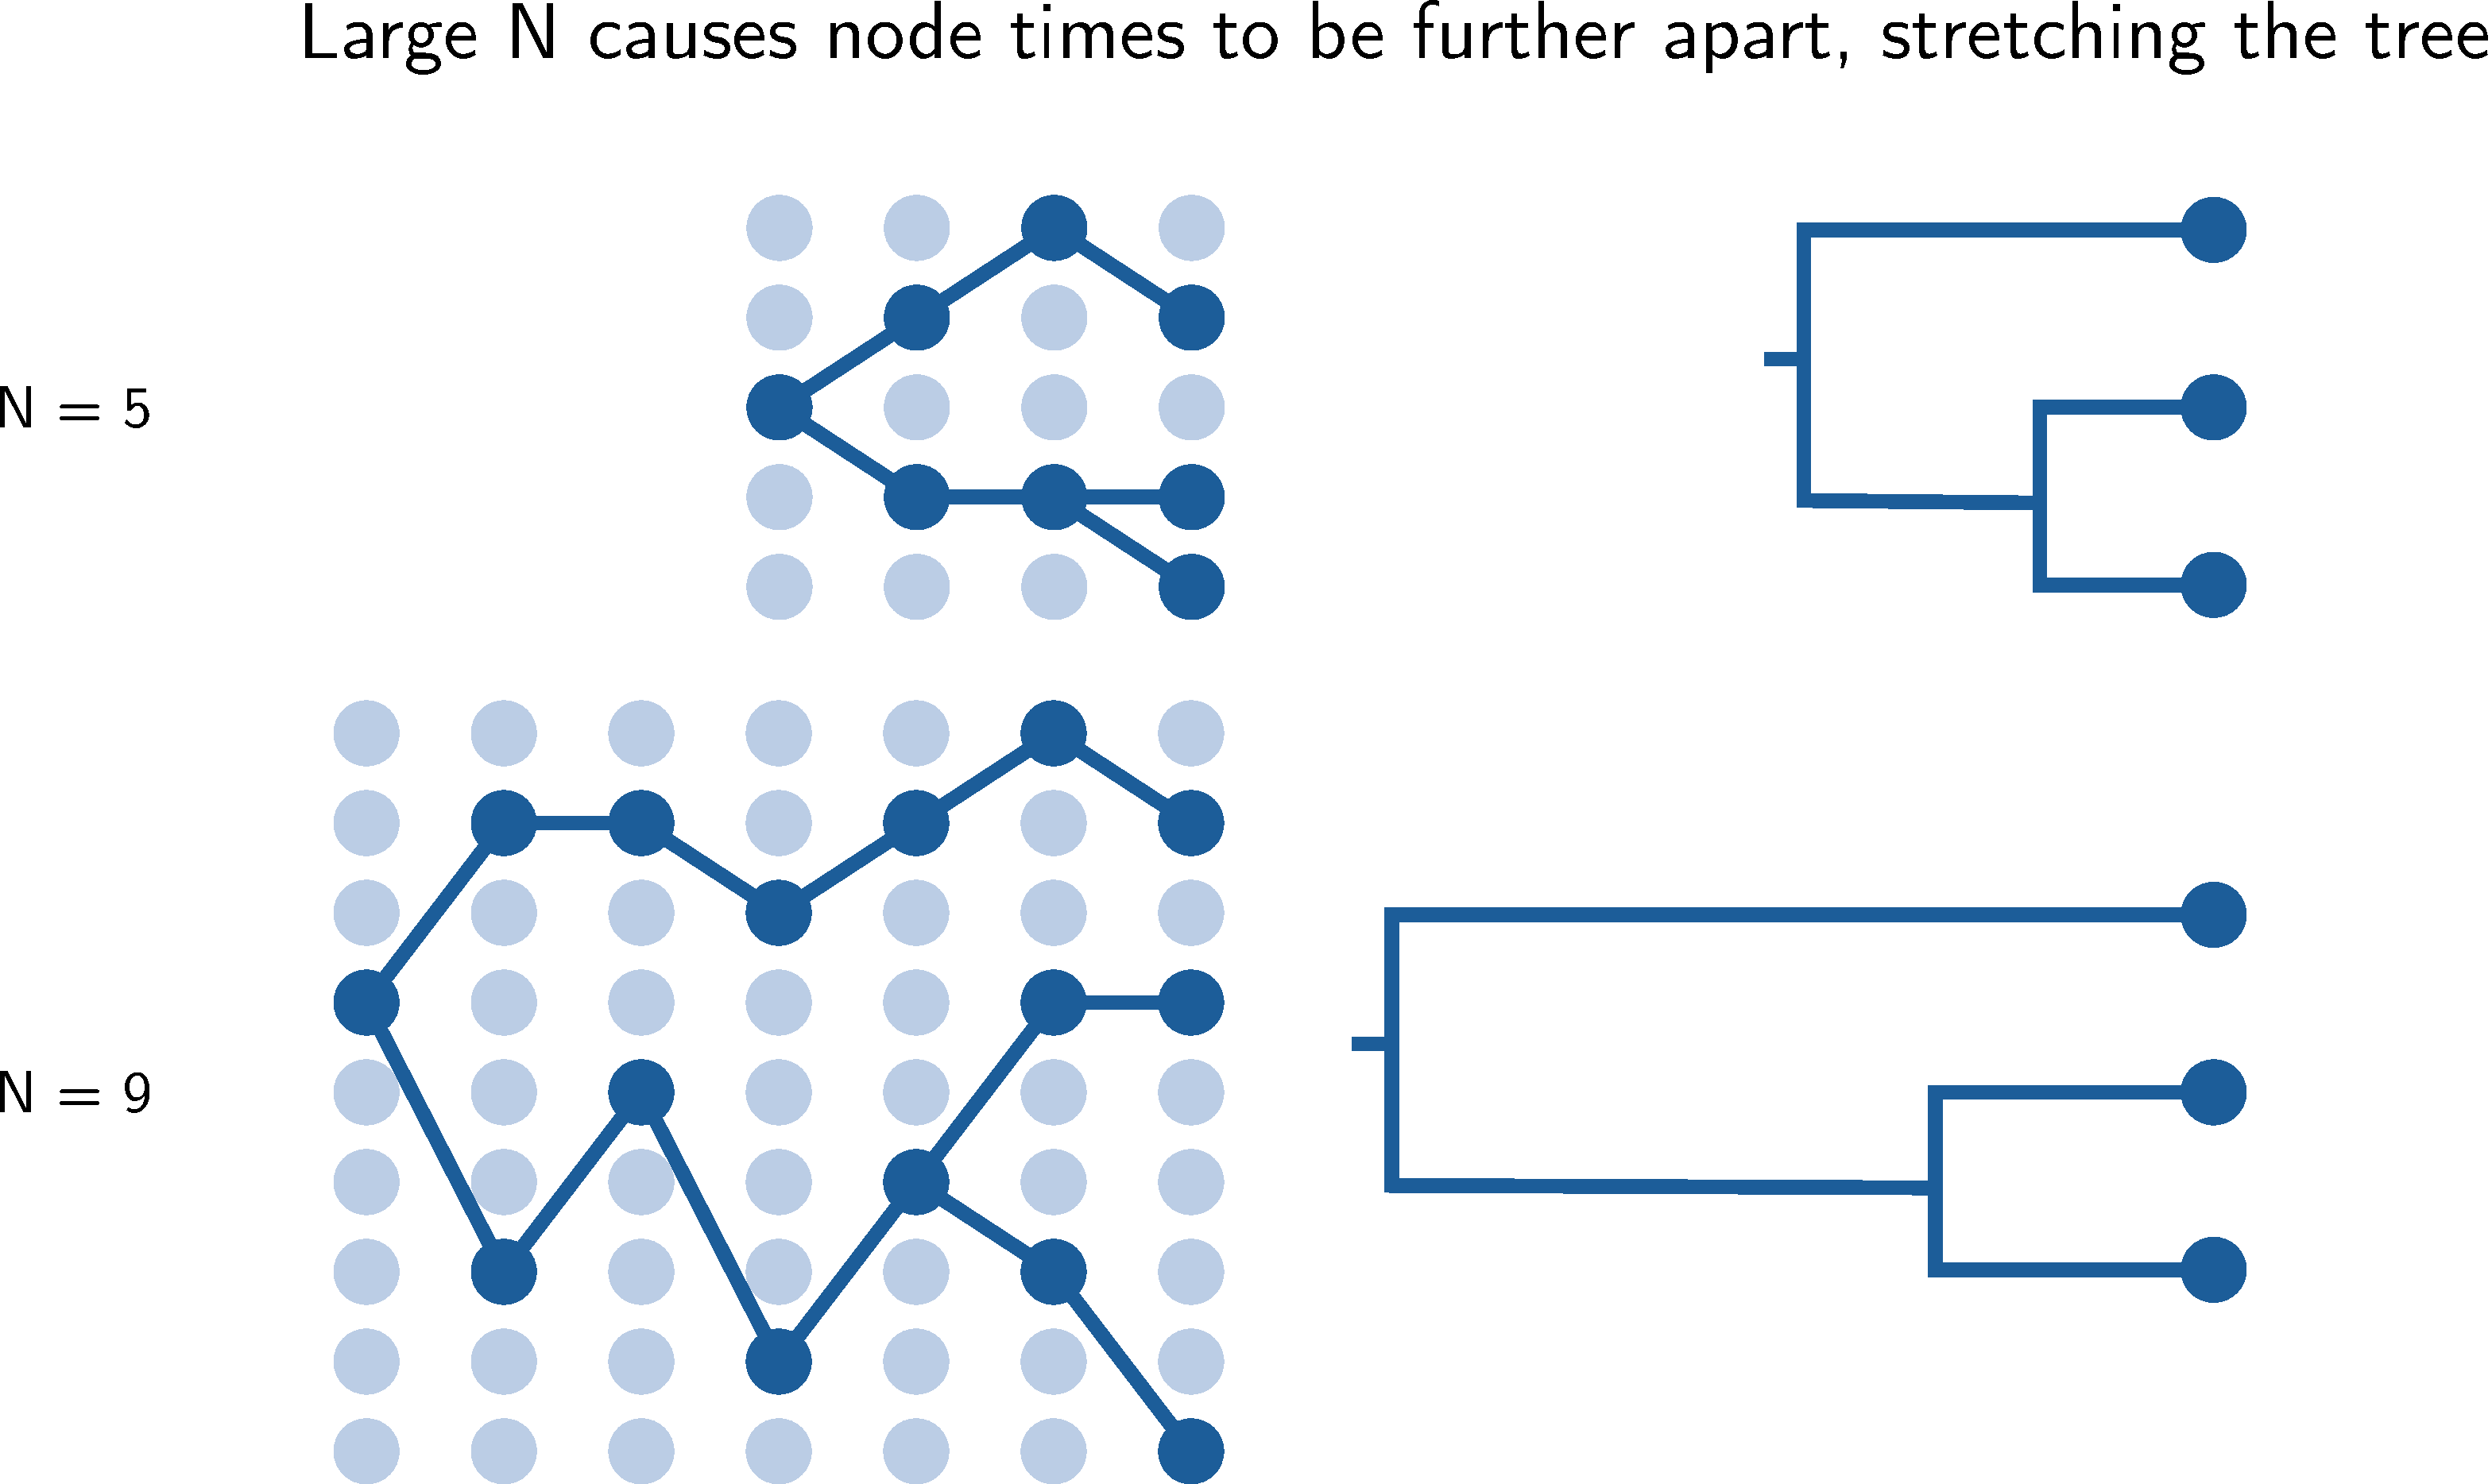
\includegraphics[width=0.8\textwidth]{images/coalescence}
        

\end{frame}

%--------------------------------------------------
\section{Effect of different linear populations}
%--------------------------------------------------

\begin{frame} \frametitle{\insertsection}

    \vspace{0.18cm}

    \centering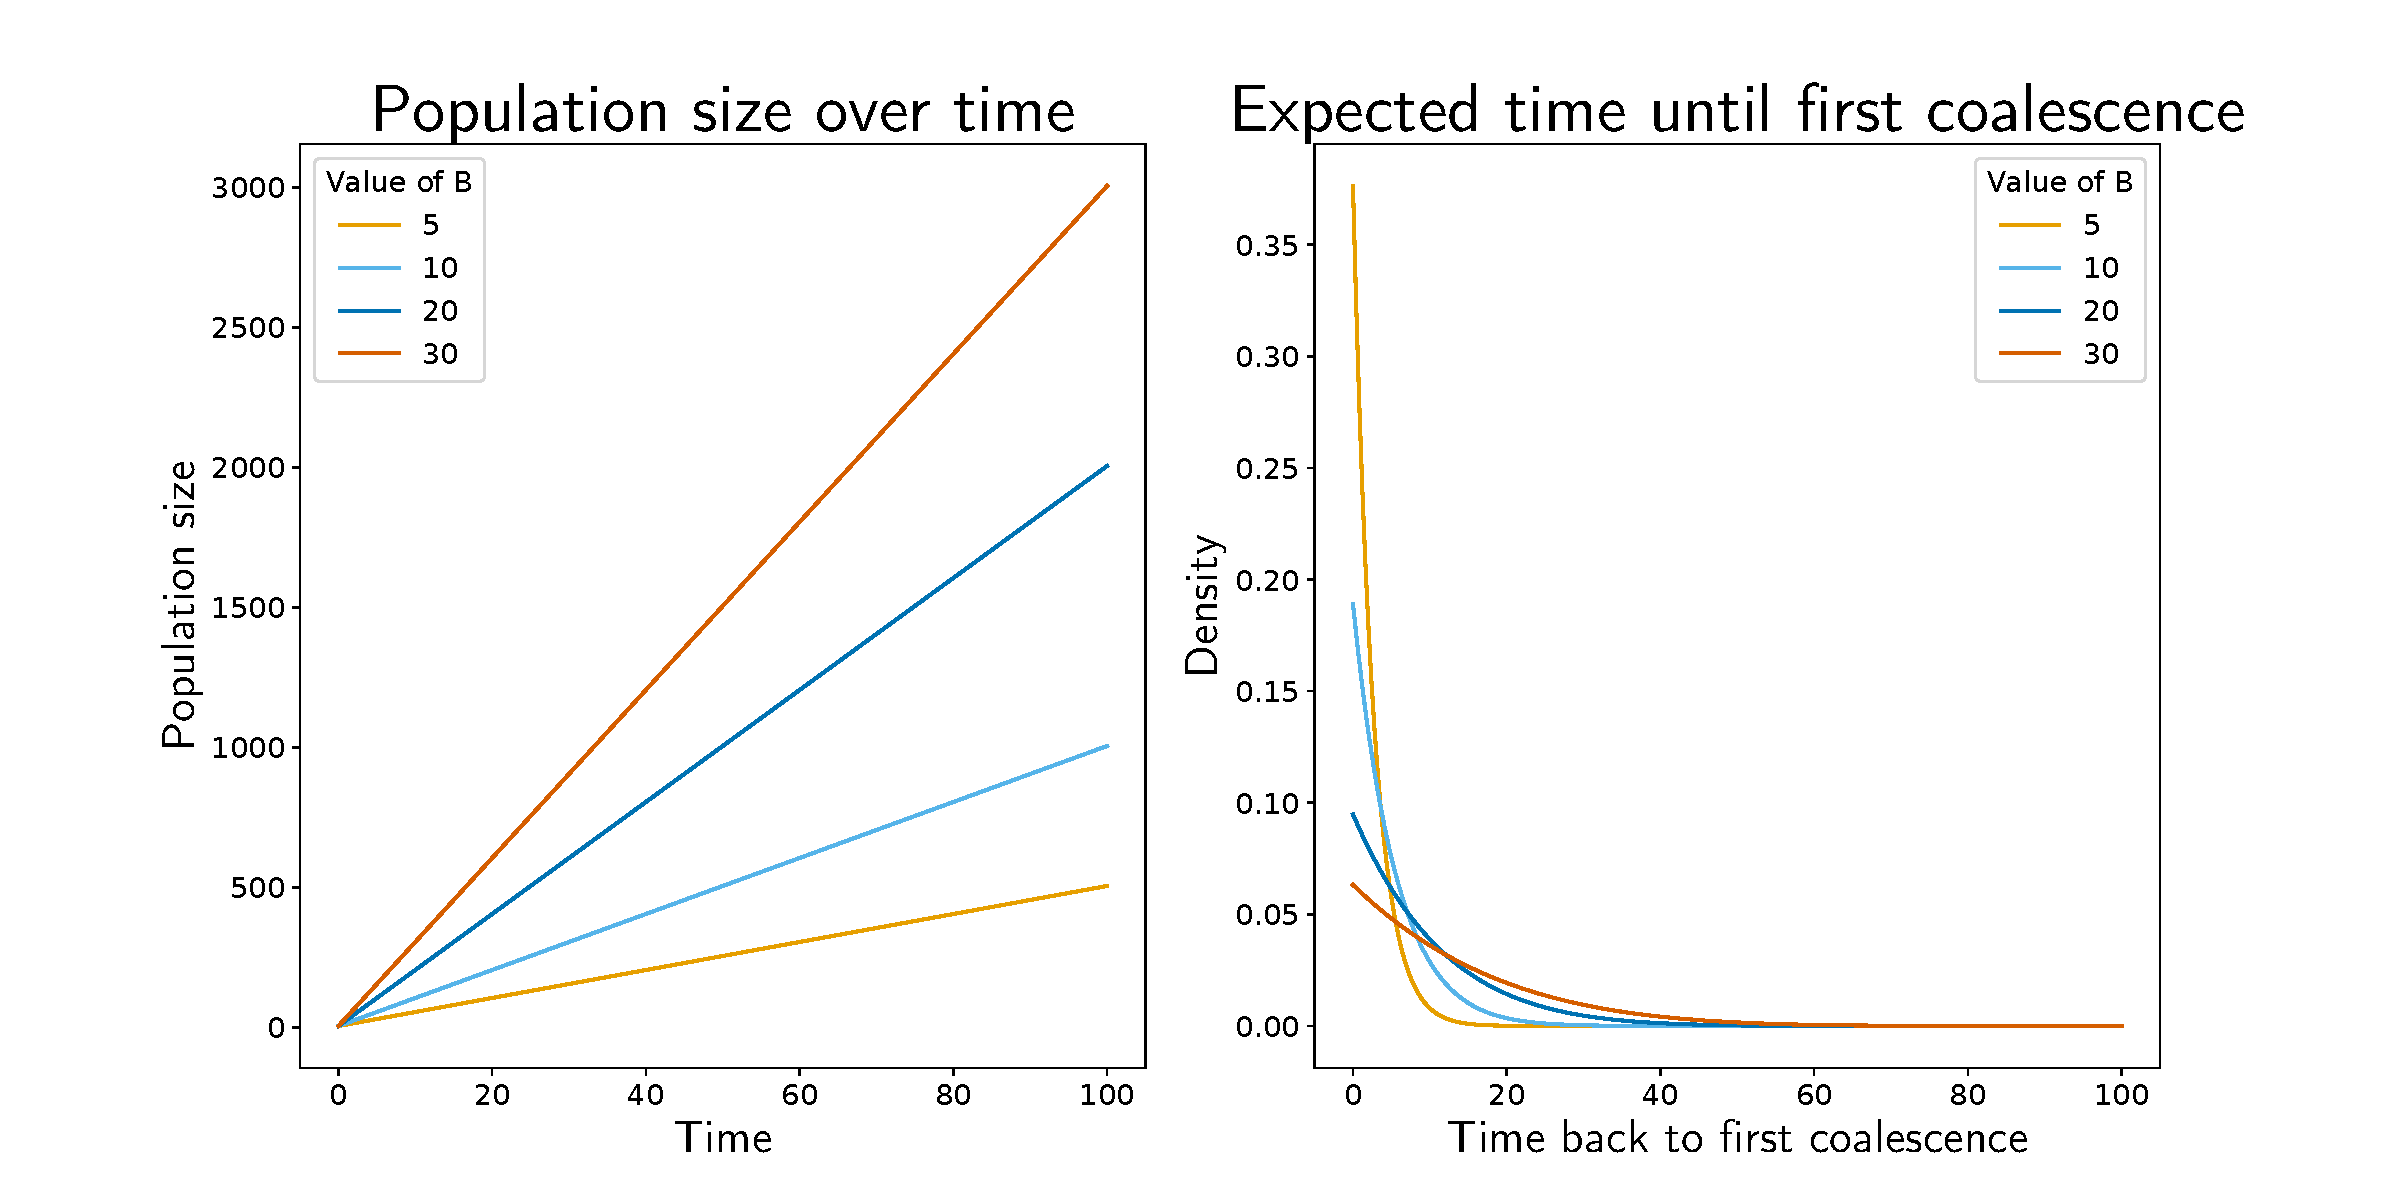
\includegraphics[width=\textwidth]{images/several-b}
        
    \ftnB{Romero-Severson et al., Mol. Biol. Evol. (2014); Shankarappa et al., Jrnl. Virology (1999); Zanini et al., eLife (2015)}

\end{frame}

%-------------------------------------------------
\section{Finding the likelihood of a whole tree}
%-------------------------------------------------

\begin{frame} \frametitle{\insertsection}

    \centering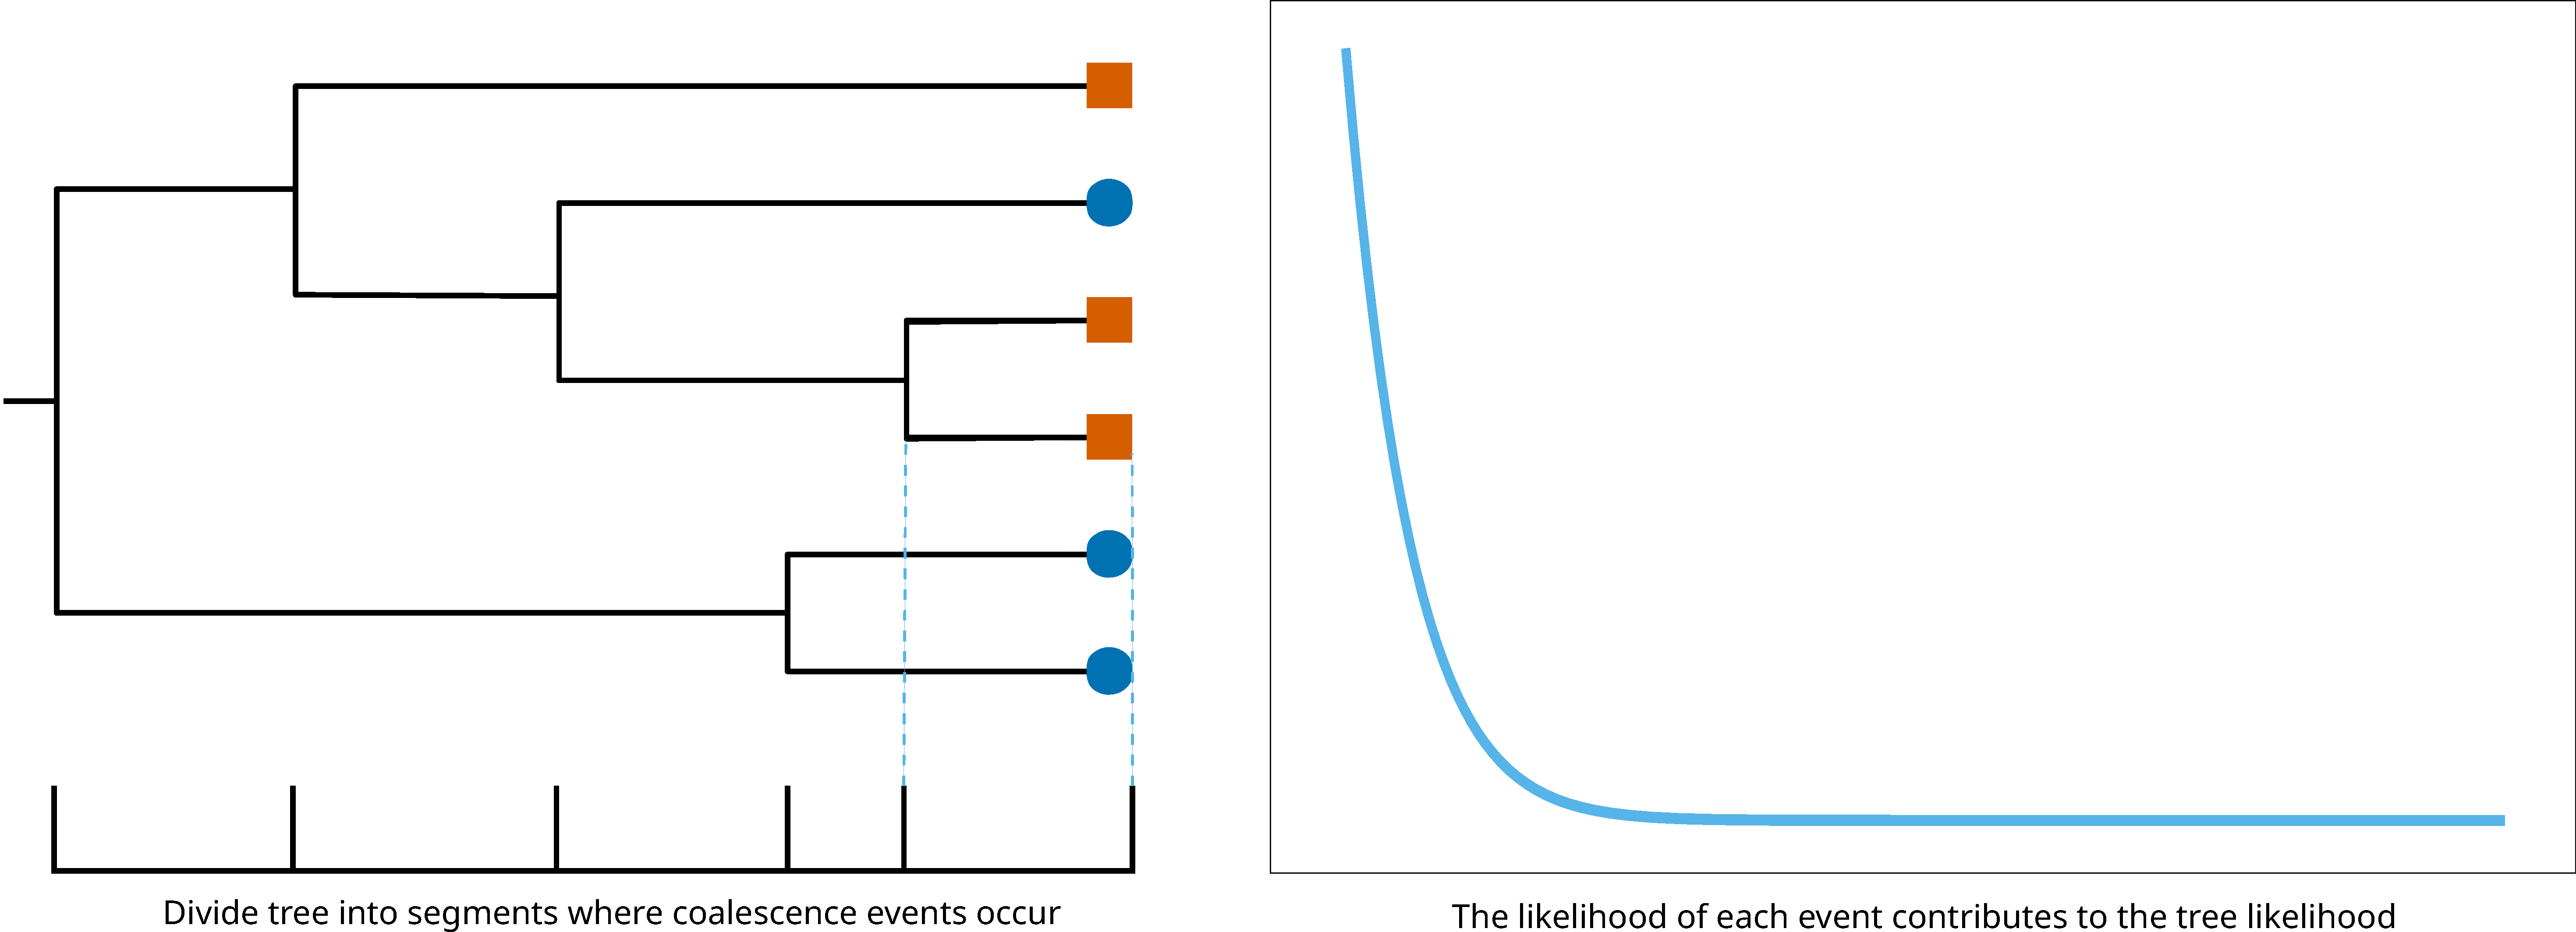
\includegraphics[width=\textwidth]{images/tree-likelihood}

\end{frame}

%--------------------------------------------------
\section{Predicting transmission time on a changing population}
%--------------------------------------------------

\begin{frame} \frametitle{\insertsection}

    \centering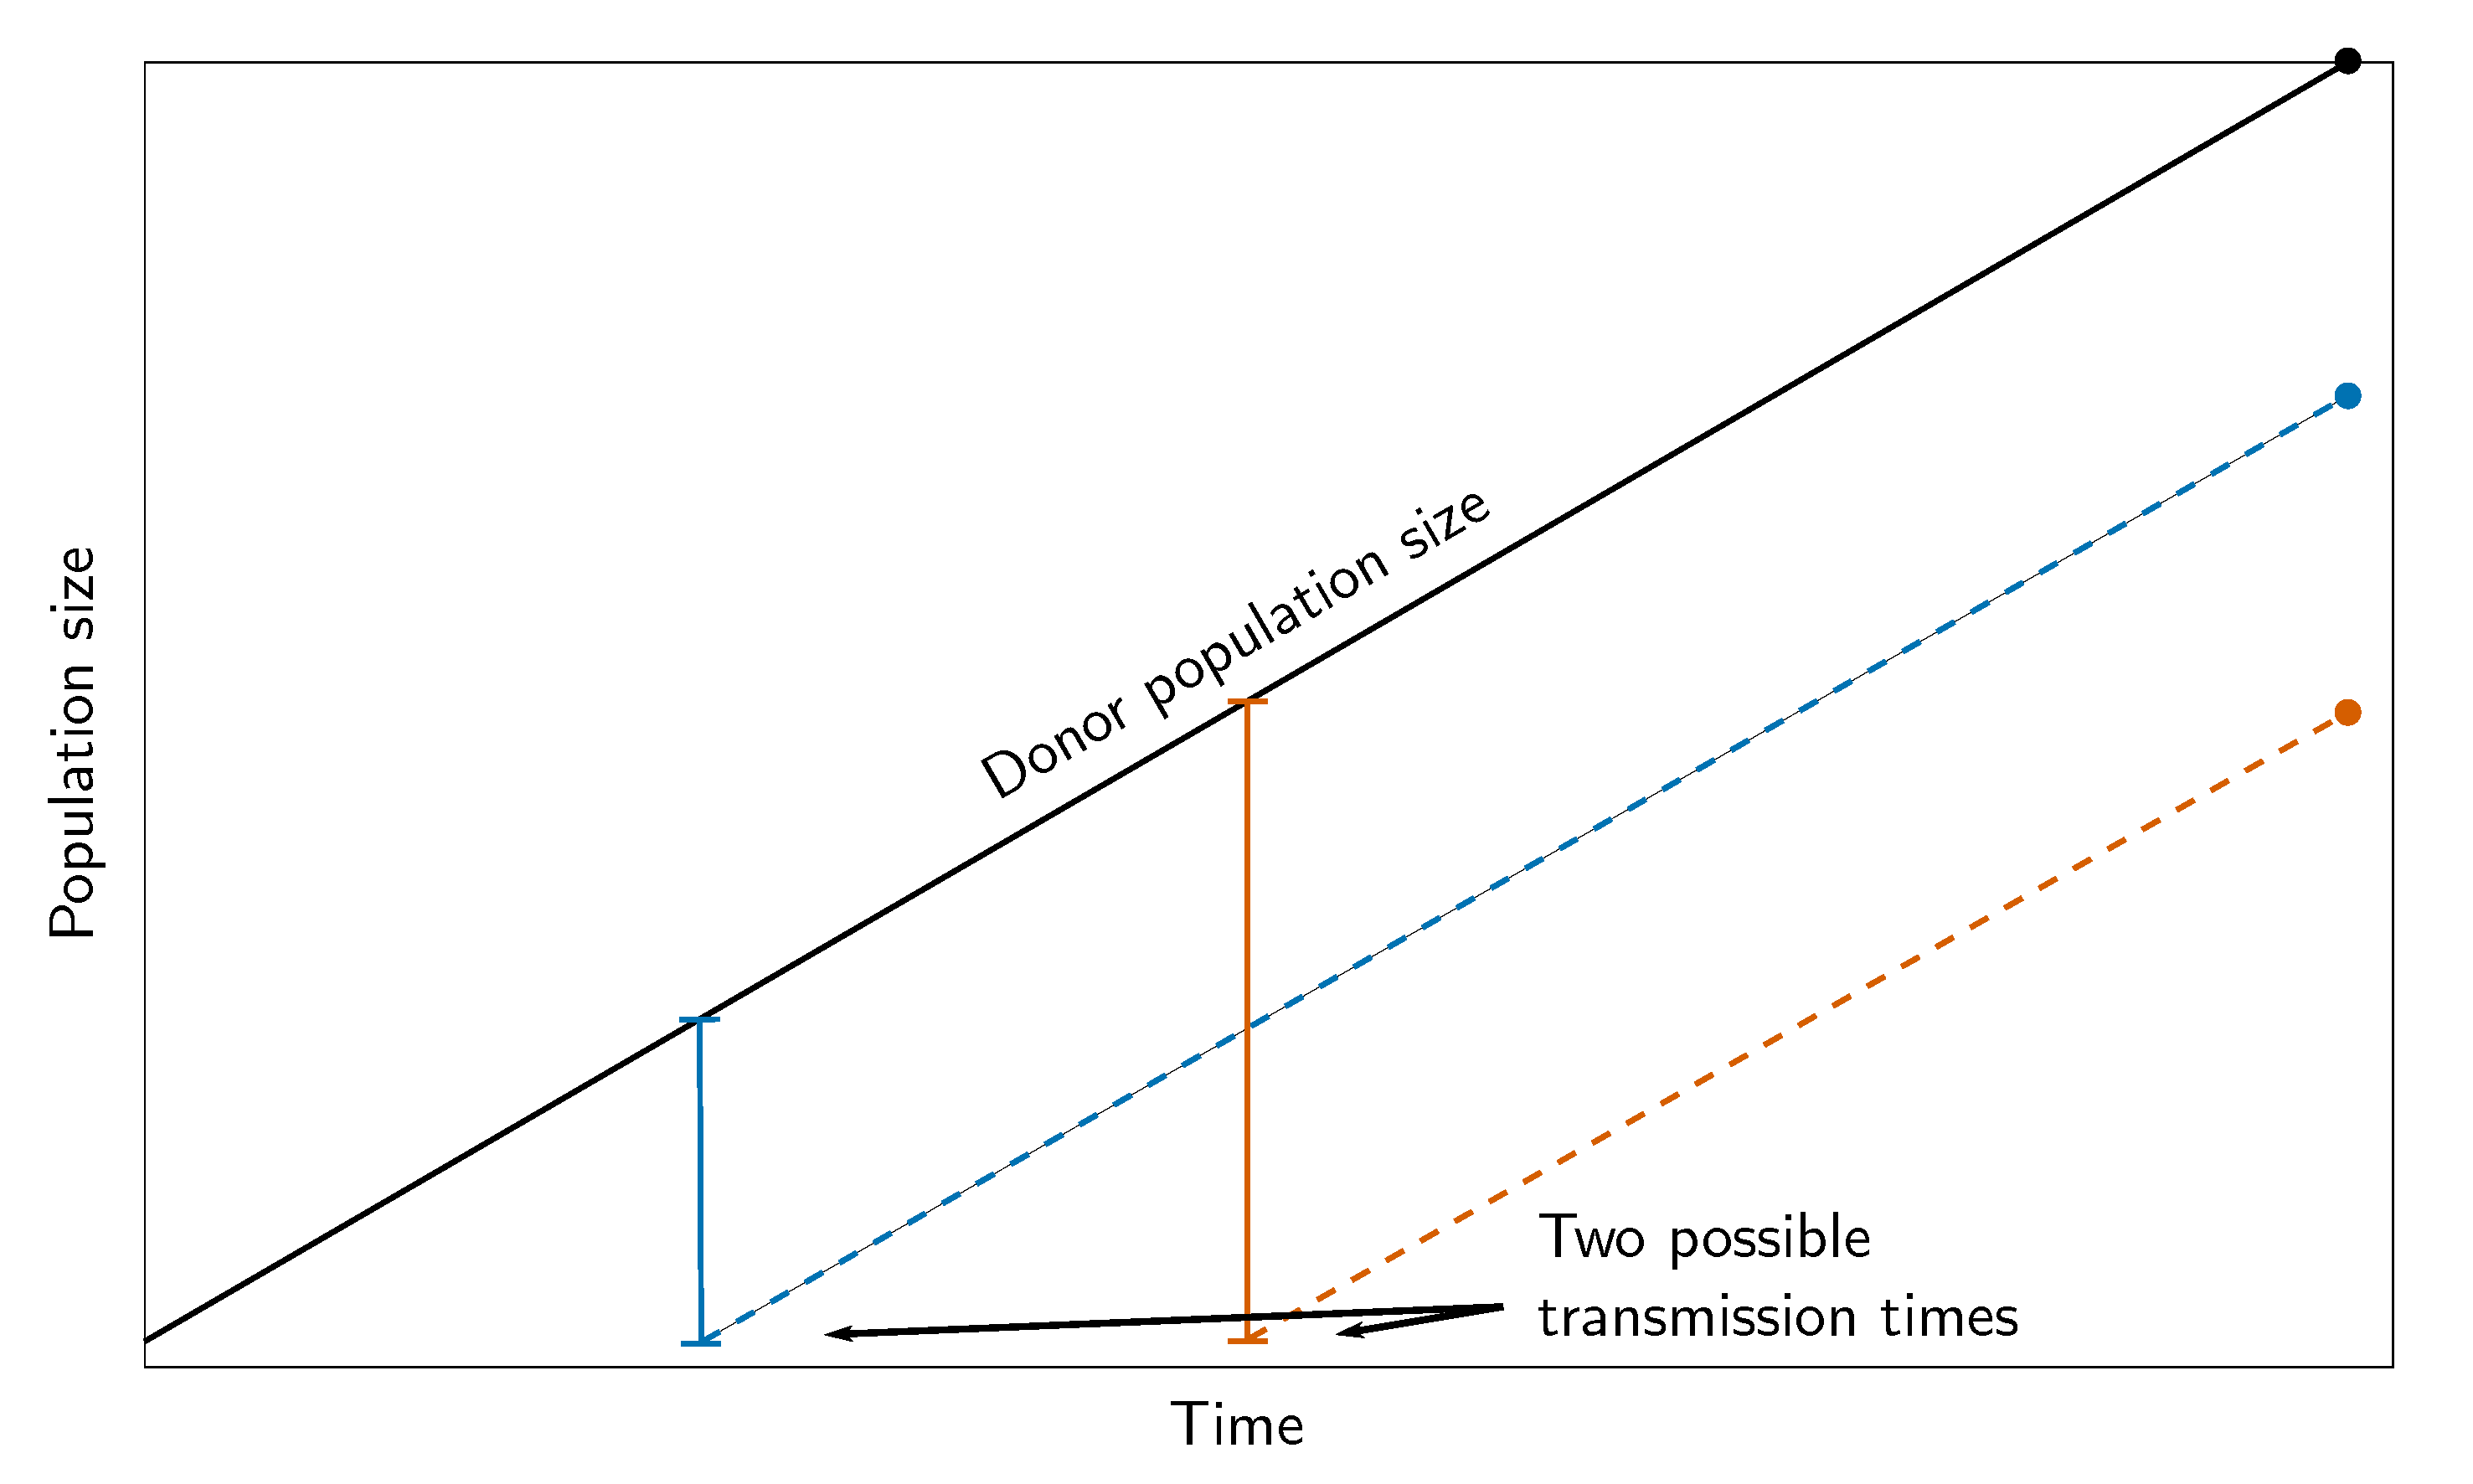
\includegraphics[width=0.8\textwidth]{images/linear-time-location}

\end{frame}

%--------------------------------------------------
\section{Results: Single host with constant population}
%--------------------------------------------------

\begin{frame} \frametitle{\insertsection}

    \centering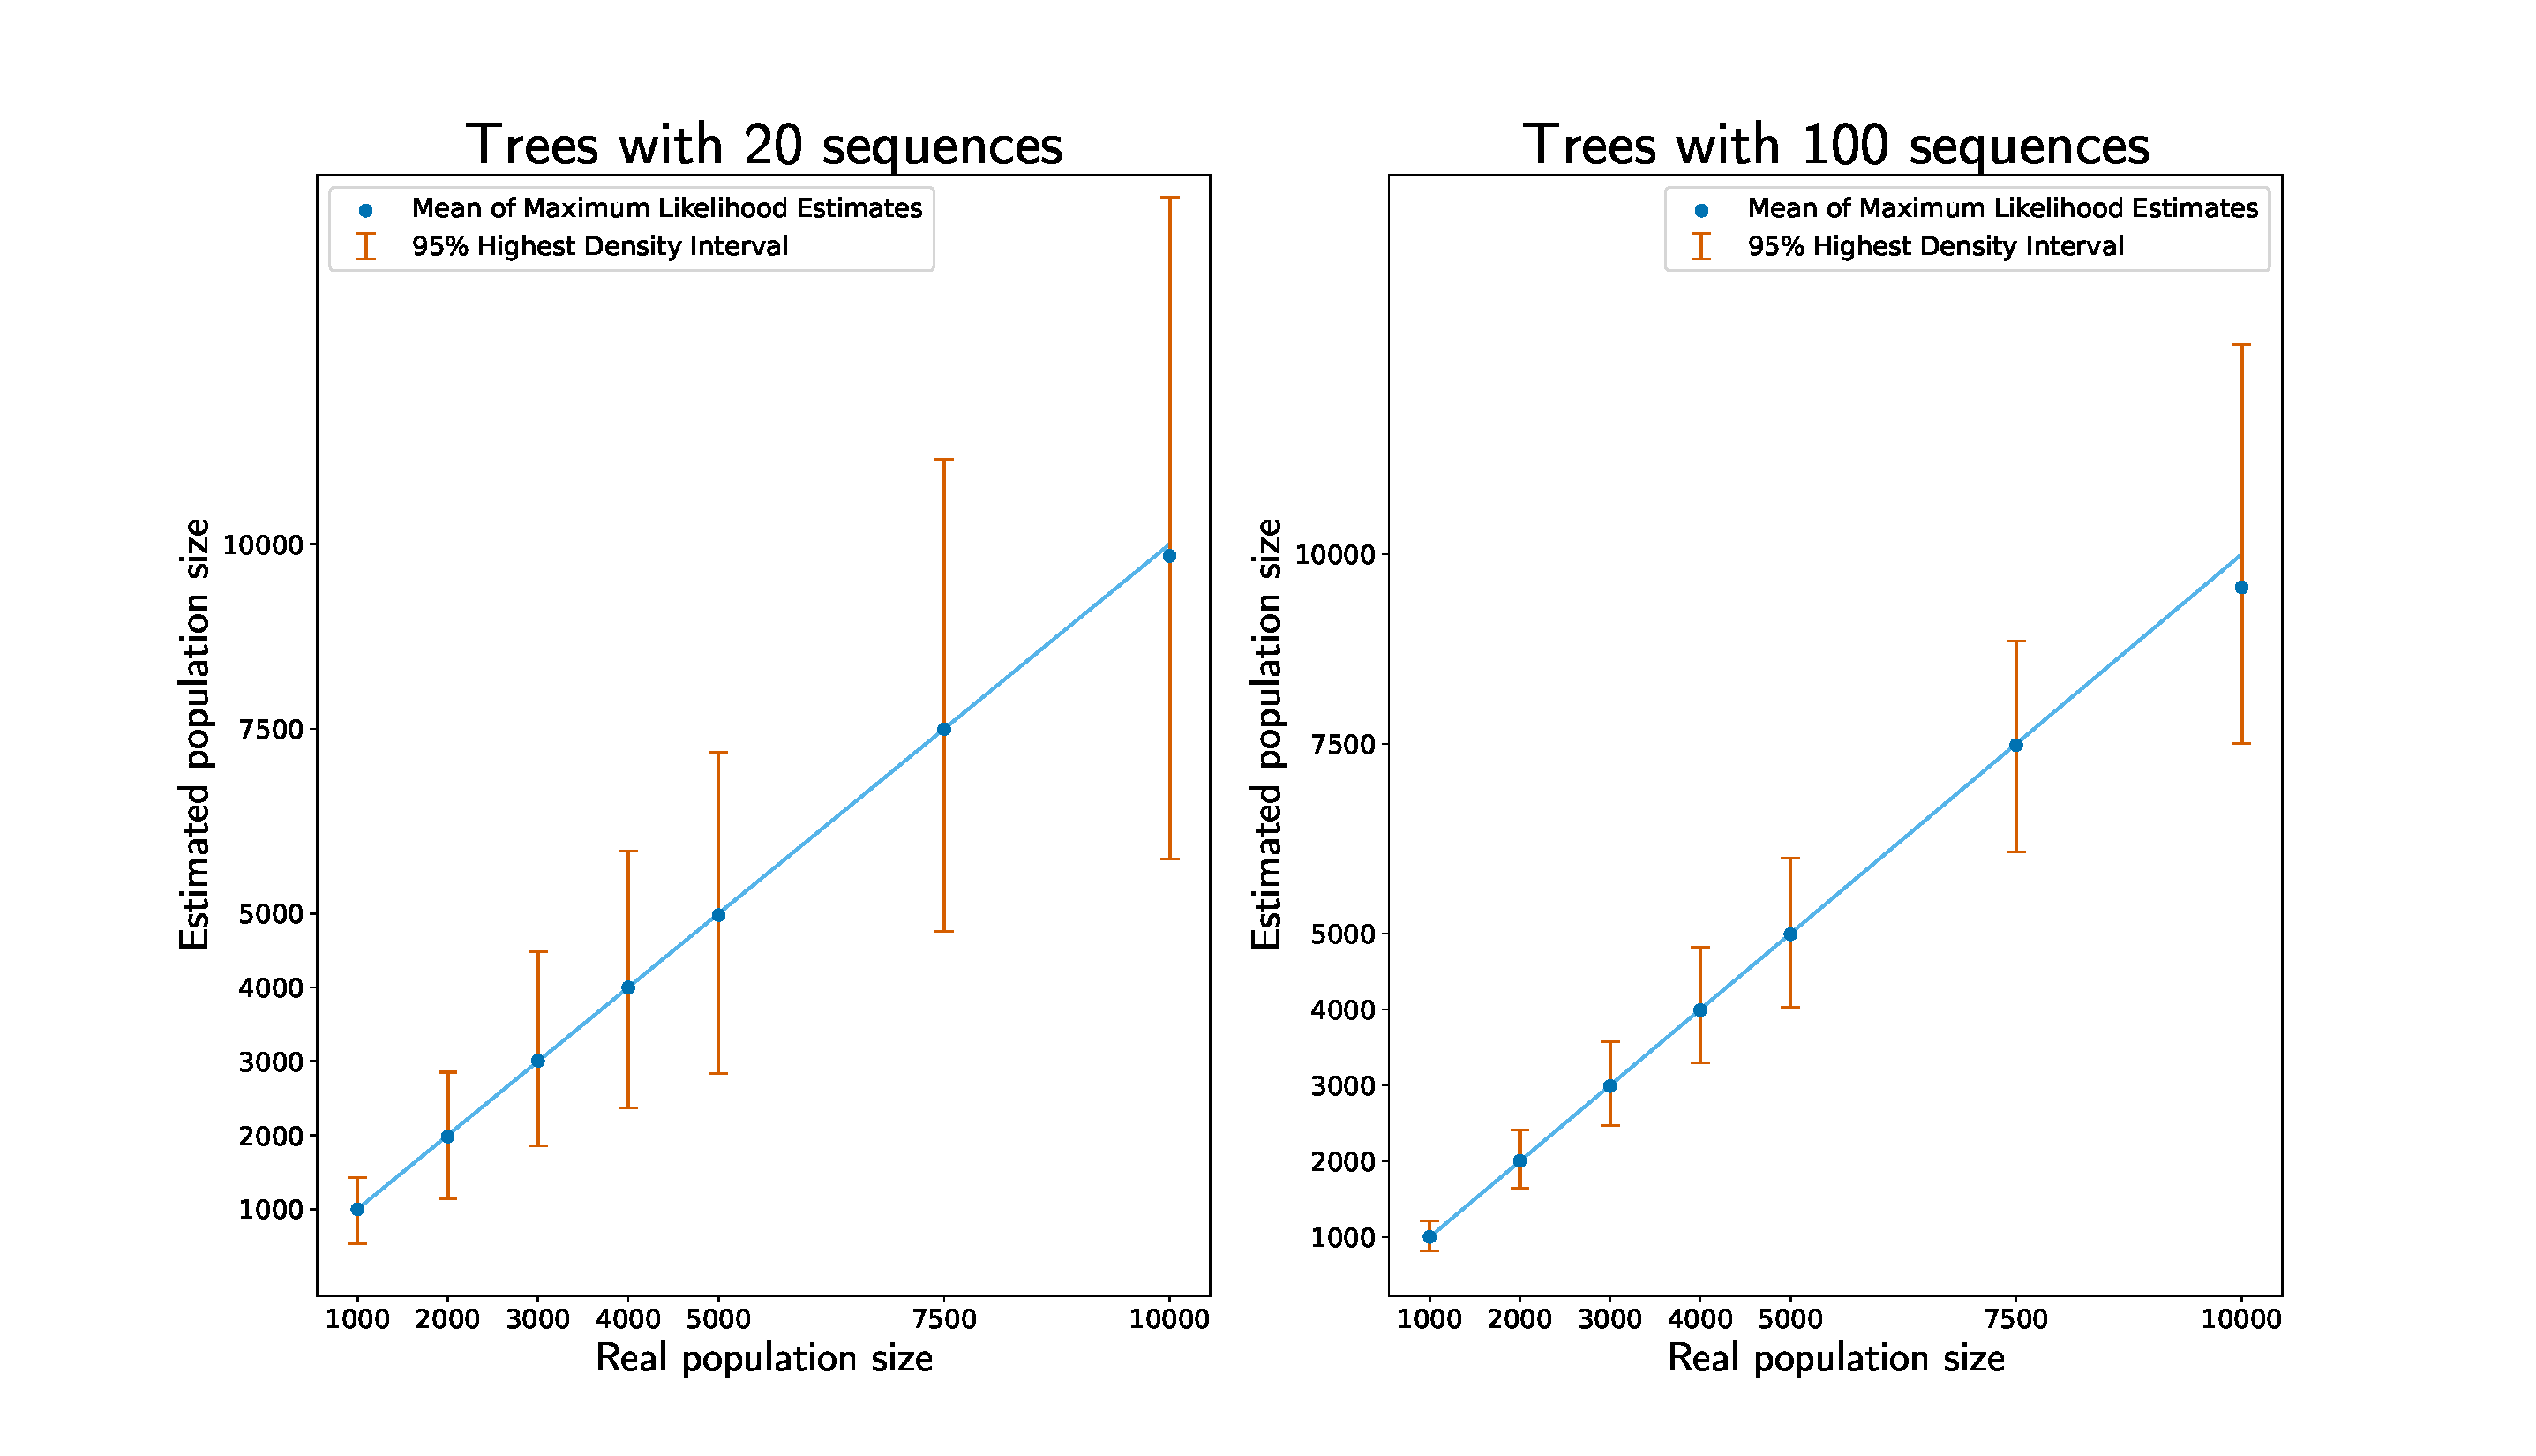
\includegraphics[width=\textwidth]{images/constant-accuracy}

\end{frame}

%---------------------------------------------------
\section{Current progress on linear populations}
%---------------------------------------------------

\begin{frame} \frametitle{\insertsection}

    \centering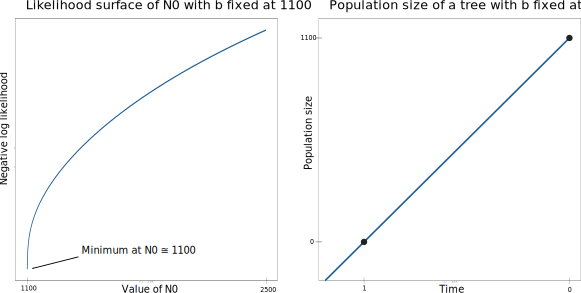
\includegraphics[width=\textwidth]{images/linear-progress}

\end{frame}

%--------------------------------------------------
\section{Next steps: Two hosts with linear population}
%--------------------------------------------------

\begin{frame} \frametitle{\insertsection}
    
    \begin{columns}

        \begin{column}{0.5\textwidth}

            \textbf{Immediately:} Solve numerical issues with linear optimization 

            \textbf{Immediately:} Extend my current work to trees with multiple hosts

            \begin{itemize}
                \item{Split tree by host}
                \item{Isolate hosts until a transmission occurs}
            \end{itemize}
            
        \end{column}

        \begin{column}{0.5\textwidth}

            \centering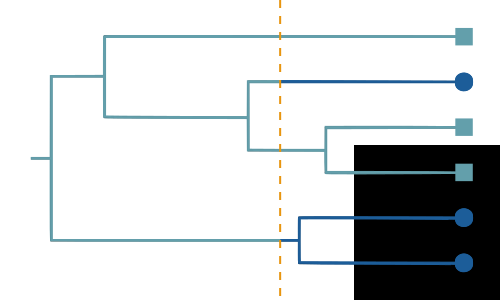
\includegraphics[width=\textwidth]{images/tree-option1}

        \end{column}

    \end{columns}
    
    \vfill

    \textbf{Overall:} Find the most likely time of transmission for phylogenetic
    trees under a range of conditions 

\end{frame}

\begin{frame}

    \begin{center}

        \begin{Huge}

            Thank you!

        \end{Huge}

        % I thought maybe I could put some more info here, but I also don't need to IDK

    \end{center}

\end{frame}

\end{document}
